\documentclass[conference]{IEEEtran}

\usepackage{cite}
\usepackage{amsmath,amssymb}
\usepackage{graphicx}
\usepackage{booktabs}
\usepackage{array}
\usepackage{tabularx}
\usepackage{tikz}
\usepackage{xcolor}
\usepackage{url}

\usetikzlibrary{arrows.meta,positioning}

\newcolumntype{Y}{>{\raggedright\arraybackslash}X}
\newcolumntype{L}[1]{>{\raggedright\arraybackslash}p{#1}}

\title{From Repeated Corrosion Images to Proxy-RUL Screening:\\An Interpretable Feasibility Pipeline for Ferrocement Specimens}

\author{\IEEEauthorblockN{Parastoo Hashemi Alvar}
\IEEEauthorblockA{\textit{Politecnico di Torino} \\
s339438 \\
s339438@studenti.polito.it}
}

\begin{document}

\maketitle

\begin{abstract}
This paper presents a multi-stage pipeline that uses repeated corrosion images of ferrocement specimens to quantify visible corrosion, estimate hidden structural condition, and generate threshold-based proxy-RUL screening outputs. The study was motivated by a clear imbalance in the available data: visible corrosion labels exist for all 792 image observations, whereas structural measurements exist for only 48 late-stage rows, one per specimen. The repository therefore does not support direct supervised remaining useful life prediction. Instead, the implemented workflow reconstructs a specimen-by-time datset, then preprocesses each image, extracts interpretable corrosion descriptors, predicts visible corrosion severity, estimates hidden structural condition, fits specimen-level degradation curves, and finally computes the time to future engineering threshold crossing as a proxy remaining useful life. The image-analysis stage extracts 91 interpretable features describing corrosion amount, location, morphology, color, and texture. In the saved grouped specimen-holdout split, the best visible-corrosion models achieved mean absolute error of 1.38 for total rust and 4.21 for peak rust, improving the previously documented peak-rust baseline. Hidden-damage estimation remained feasible but much weaker, with mean absolute error of 3.90 for wire-area loss and 0.121~kN for ultimate load, and it degraded sharply under campaign and treatment holdouts. Degradation fitting produced 192 curves and 52{,}416 forecast rows, with piecewise-linear fits dominating. The final remaining-life outputs are screening-only quantities derived from forecasted threshold crossing, not true lifetime predictions. The strongest validated result of the repository is therefore image-based visible corrosion estimation; the structural and proxy-RUL layers are mixed-input feasibility extensions limited by sparse supervision and propagated uncertainty.
\end{abstract}

\begin{IEEEkeywords}
corrosion assessment, ferrocement, hidden damage, degradation modeling, proxy remaining useful life, interpretable image features
\end{IEEEkeywords}

\section{Introduction}
Visible corrosion is often the earliest measurable sign of deterioration. Rust patches, local darkening, and changes in color or texture can be observed directly in images, which makes image-based monitoring attractive for repeated inspection. The engineering goal, however, is not only to describe surface appearance. The larger question is whether visible corrosion can support conclusions about hidden structural condition, future deterioration, and remaining service margin.

That question becomes difficult when the dataset is uneven in what it observes. In this repository, image observations are dense and repeated over time, but structural measurements are sparse and appear only at late stages.

The dataset does not contain true failure times, so the paper does not claim direct image-to-life prediction. Instead, it documents a staged feasibility pipeline:

\begin{center}
raw observations $\rightarrow$ clean specimen histories $\rightarrow$ image-derived corrosion descriptors $\rightarrow$ visible corrosion state $\rightarrow$ hidden structural estimate $\rightarrow$ degradation trend $\rightarrow$ proxy remaining useful life
\end{center}

This is the central identity of the paper. It is a feasibility study of a multi-stage corrosion-to-condition workflow under sparse structural supervision.

\section{Problem Statement and Scientific Scope}
The problem addressed in this repository is not ``predict remaining life directly from images.'' The implemented problem is narrower and more defensible: use repeated corrosion images, specimen metadata, and sparse late-stage structural supervision to build a condition-assessment pipeline that ends in threshold-based screening outputs.

The paper therefore asks four questions:
\begin{enumerate}
    \item Can visible corrosion be estimated reliably from image-derived descriptors?
    \item Can visible corrosion and specimen metadata support estimation of hidden structural quantities?
    \item Can repeated specimen observations be summarized by degradation curves that are usable for short-horizon forward screening?
    \item Can those forecasts be converted into proxy-RUL and risk categories without overstating them as true lifetime predictions?
\end{enumerate}

Two scope boundaries are central. First, the strongest validated result in the repository is image-based visible corrosion modeling, because that stage has dense supervision. Second, the structural, degradation, and proxy-RUL stages are progressively weaker because they depend on only 48 structural labels, then on model-estimated states, and finally on forecasted threshold crossing.

\section{Dataset and Evidence Structure}
The dataset contains 792 image observations from 48 specimens across 2 campaigns, covering 25 observed week values from week 0 to week 36. Each row contains specimen identity, observation time, one corrosion image, specimen and exposure metadata, and visible corrosion labels. Structural supervision is far sparser: 48 rows contain structural measurements, corresponding to one late-stage structural row per specimen at weeks 28 and 36 only.

\begin{table}[t]
    \caption{Dataset Summary}
    \label{tab:dataset-summary}
    \centering
    \small
    \begin{tabular}{lr}
        \toprule
        Quantity & Value \\
        \midrule
        Image observations & 792 \\
        Specimens & 48 \\
        Campaigns & 2 \\
        Week range & 0 to 36 \\
        Unique observed week values & 25 \\
        Surface-labeled rows & 792 \\
        Structural-labeled rows & 48 \\
        Structural-label coverage & 6.06\% \\
        \bottomrule
    \end{tabular}
\end{table}

A multi-stage paper becomes hard to interpret unless the evidence status of each quantity is explicit. Table~\ref{tab:evidence-structure} distinguishes what is measured, what is model-estimated, what is forecasted, and what is only a screening output.

\begin{table}[t]
    \caption{Evidence Structure of the Pipeline}
    \label{tab:evidence-structure}
    \centering
    \scriptsize
    \setlength{\tabcolsep}{3pt}
    \begin{tabular}{@{}L{0.28\linewidth}L{0.26\linewidth}L{0.38\linewidth}@{}}
        \toprule
        Evidence class & Examples & Meaning in this study \\
        \midrule
        Observed on all rows & total rust, peak rust, peak-rust location & Direct surface-corrosion supervision \\
        Observed on 48 late-stage rows & wire-area loss, ultimate load & Sparse structural supervision \\
        Model-estimated on all rows & estimated wire loss, estimated ultimate load & Latent structural state inferred from the damage stage \\
        Forecasted & degradation trajectories, threshold-crossing times & Extrapolated future states from fitted curves \\
        Derived screening outputs & proxy-RUL, failure proxy, risk class & Screening-only outputs, not observed failure outcomes \\
        \bottomrule
    \end{tabular}
\end{table}

The dataset supports repeated observation of visible corrosion, specimen-level time-series reconstruction, image-based corrosion modeling, preliminary hidden-damage estimation, and threshold-based screening. It does not support direct supervised prediction of true remaining useful life because failure times are not observed.

\begin{figure*}[t]
    \centering
    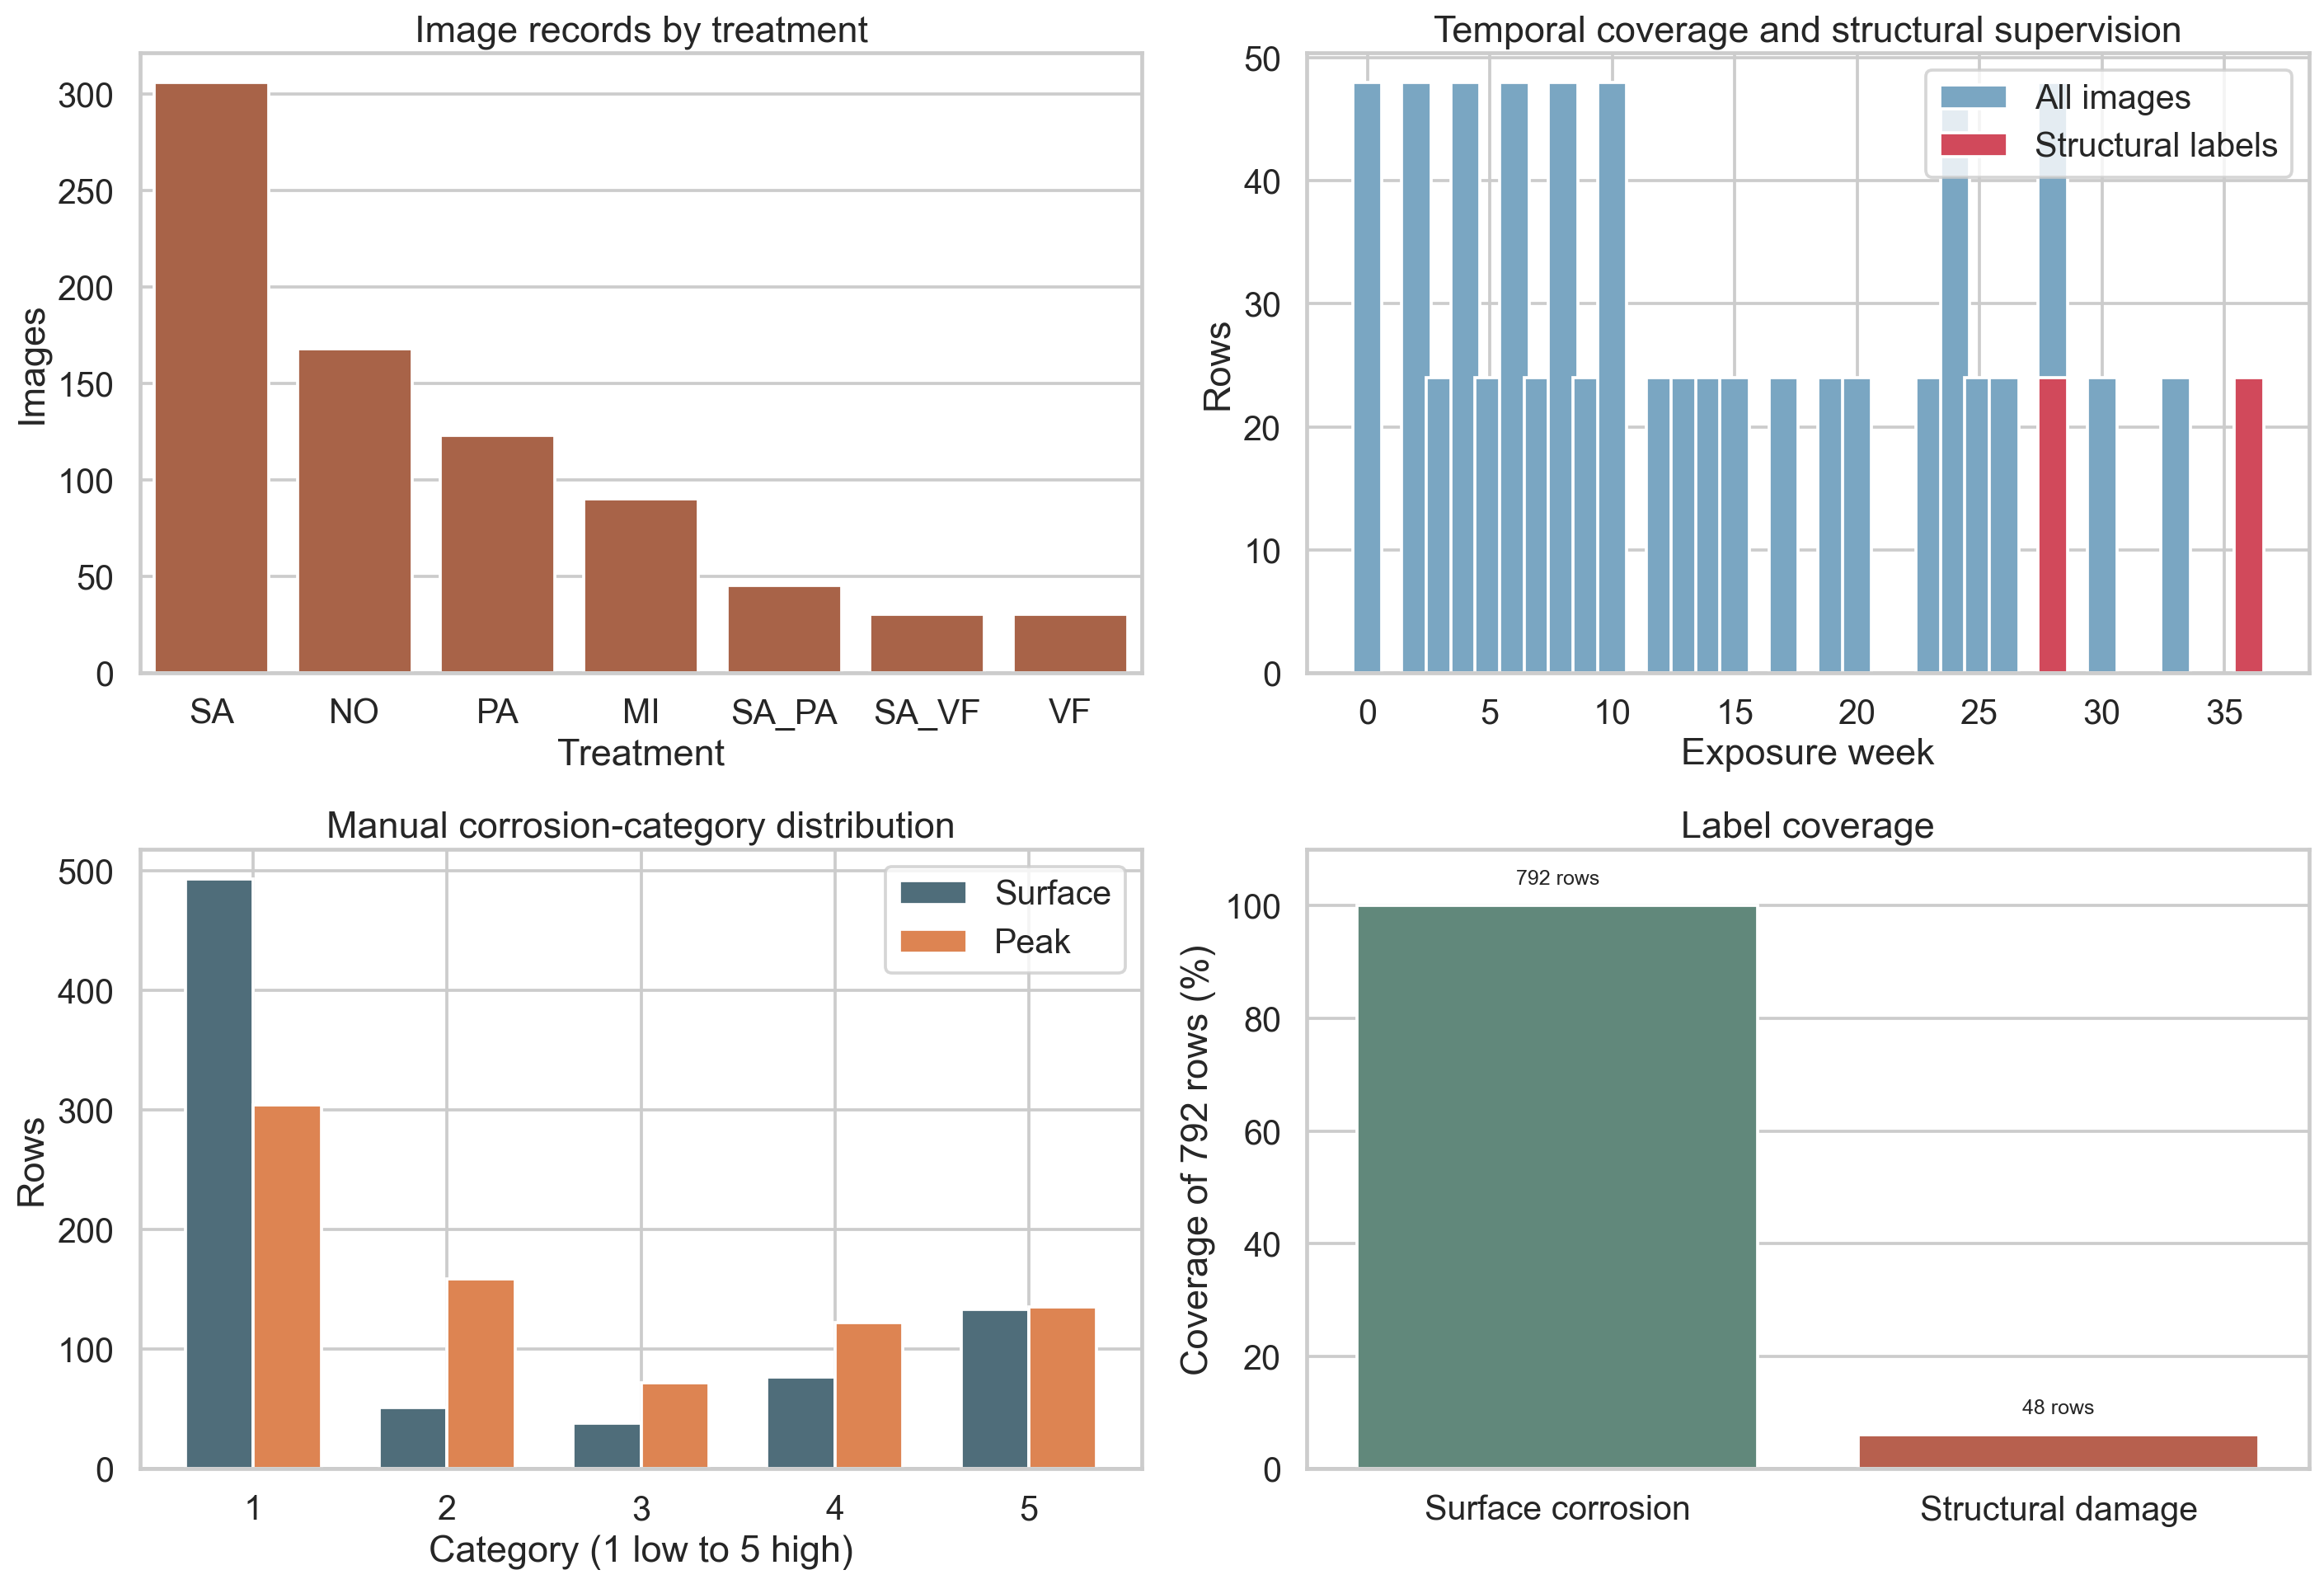
\includegraphics[width=0.96\textwidth]{meeting_report/figures/dataset_overview.png}
    \caption{Dataset overview used in the study. The upper panels summarize image-record counts by treatment and by exposure week, while the lower panels show manual corrosion-category distributions and label coverage. The lower-right panel highlights the central data imbalance that motivates the staged pipeline: surface labels exist for all 792 rows, whereas structural supervision exists for only 48 late-stage rows.}
    \label{fig:dataset-overview}
\end{figure*}

\section{End-to-End Pipeline Overview}
The workflow was designed as a chain of connected stages. Each stage has a clear input, performs one specific transformation, and produces an output that becomes the input of the next stage.

\begin{figure*}[t]
    \centering
    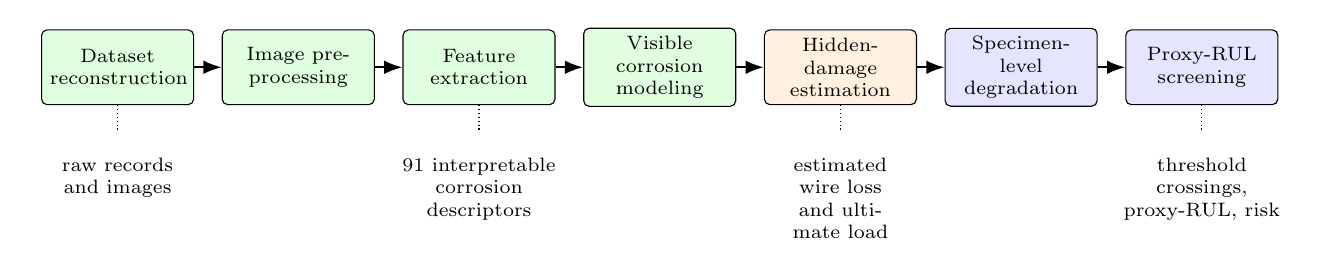
\begin{tikzpicture}[
        >=Latex,
        node distance=0.35cm,
        every node/.style={font=\scriptsize, align=center},
        stage/.style={draw, rounded corners=2pt, minimum height=0.95cm, text width=1.72cm, inner sep=3pt},
        observed/.style={stage, fill=green!12},
        estimated/.style={stage, fill=orange!12},
        forecast/.style={stage, fill=blue!10}
    ]
        \node[observed] (s1) {Dataset\\reconstruction};
        \node[observed, right=of s1] (s2) {Image pre-\\processing};
        \node[observed, right=of s2] (s3) {Feature\\extraction};
        \node[observed, right=of s3] (s4) {Visible corrosion\\modeling};
        \node[estimated, right=of s4] (s5) {Hidden-damage\\estimation};
        \node[forecast, right=of s5] (s6) {Specimen-level\\degradation};
        \node[forecast, right=of s6] (s7) {Proxy-RUL\\screening};

        \draw[->, thick] (s1) -- (s2);
        \draw[->, thick] (s2) -- (s3);
        \draw[->, thick] (s3) -- (s4);
        \draw[->, thick] (s4) -- (s5);
        \draw[->, thick] (s5) -- (s6);
        \draw[->, thick] (s6) -- (s7);

        \node[below=0.55cm of s1, text width=2.05cm] {raw records\\and images};
        \node[below=0.55cm of s3, text width=2.15cm] {91 interpretable\\corrosion descriptors};
        \node[below=0.55cm of s5, text width=2.15cm] {estimated wire loss\\and ultimate load};
        \node[below=0.55cm of s7, text width=2.15cm] {threshold crossings,\\proxy-RUL, risk};

        \draw[densely dotted] (s1.south) -- ++(0,-0.32);
        \draw[densely dotted] (s3.south) -- ++(0,-0.32);
        \draw[densely dotted] (s5.south) -- ++(0,-0.32);
        \draw[densely dotted] (s7.south) -- ++(0,-0.32);
    \end{tikzpicture}
    \caption{Step-by-step workflow used in the study. Green stages operate on directly observed data, orange stages estimate hidden structural state, and blue stages forecast future condition and convert threshold crossing into screening outputs. The figure makes explicit that proxy-RUL is not predicted directly from images; it is derived only after corrosion modeling, hidden-damage estimation, and specimen-level degradation fitting.}
    \label{fig:workflow}
\end{figure*}

\section{Methodology}
\subsection{Dataset Reconstruction and Validation}
The pipeline begins with the raw spreadsheet and the PNG image directory. The spreadsheet is cleaned by treating its first row as the true header row, then its columns are renamed into a consistent schema. The record identifier is parsed using a fixed pattern of the form \texttt{specimenID-YYYYMMDD-weekW}. This yields specimen identity, capture date, and exposure week. The image directory is scanned independently, each PNG stem is treated as a record identifier, and the spreadsheet table is merged to image paths using that key.

Additional metadata are reconstructed at this stage. Treatment codes are expanded into human-readable treatment names. Campaign labels are inferred from capture year, mesh count, salt concentration, and ageing duration. A flag is created to indicate whether structural labels are available. Sequence order is assigned within each specimen history. Duplicate record IDs and duplicate specimen-week combinations are flagged explicitly.

One engineering correction is also applied here. The raw wire-loss field behaves numerically like a fraction rather than a percentage. Therefore, when its maximum value is small enough to indicate ratio storage, it is multiplied by 100 and stored as wire-area loss percentage.

This stage creates the backbone of the entire study. Without a clean specimen-wise time-series table, later stages such as degradation fitting and remaining-life screening would not be meaningful.

\subsection{Image Preprocessing and Corrosion Segmentation}
Each aligned image is opened and converted into RGB format. If an image contains transparency, it is composited onto a white background so that all images share a consistent representation.

The pipeline then extracts the central specimen region after trimming image borders and background margins. In the current implementation, the crop removes 3\% from the left, 3\% from the right, 8\% from the top, and 8\% from the bottom. This central analysis region is used because the border areas are less informative and more likely to include non-specimen background.

After cropping, illumination is normalized in two steps. First, each RGB channel is rescaled using its 2nd and 98th percentiles. Second, the brightness channel in HSV space is enhanced using adaptive histogram equalization. A rust-likelihood map is then computed by combining red dominance over green, warm-color dominance over blue, chromatic information from the Lab space, saturation in HSV space, and closeness of hue to typical red-brown corrosion tones.

The rust-likelihood map is converted into a rust mask. The threshold is chosen from the larger of Otsu's threshold and a score-based threshold equal to mean + 0.35 times standard deviation, then clipped to a stable interval. After thresholding, the mask is cleaned by removing very small objects, filling small holes, and applying small binary opening and closing operations.

A continuous rust-likelihood map is computed from red dominance over green, warm-color dominance over blue, normalized Lab chromatic channels, HSV saturation, and two hue-centered Gaussian terms around red-brown corrosion tones. Segmentation then uses
\[
\text{threshold}=\operatorname{clip}\!\left(\max(\text{Otsu},\ \mu + 0.35\sigma),\ 0.22,\ 0.82\right),
\]
followed by removal of small objects and holes, binary opening with a disk of radius 1, and binary closing with a disk of radius 2. The outputs are the cropped region of interest, the illumination-normalized RGB image, the rust-score map, the binary rust mask, and the chosen threshold.

\subsection{Interpretable Feature Extraction}
The feature extractor converts each processed image into 91 numeric descriptors. These include corrosion amount features such as rust area percentage and peak segment rust percentage; spatial features such as segment-wise corrosion and peak location; morphology features such as rust-component count and largest region area; color features in RGB, HSV, and Lab spaces; histogram summaries; and texture descriptors derived from gray-level co-occurrence matrices and local binary patterns. The specimen is divided into 12 longitudinal segments. Since the nominal specimen length is set to 24~cm, each segment corresponds to a 2~cm section, which allows the pipeline to describe where corrosion is concentrated along the specimen.

The saved feature table contains corrosion-amount features, distribution statistics, connected-component morphology, global RGB/HSV/Lab moments, 8-bin HSV histograms, and texture descriptors. Texture is computed after resizing the grayscale ROI to $96 \times 384$ pixels, building gray-level co-occurrence matrices at distances 1, 4, and 8 and angles $0^\circ$, $45^\circ$, and $90^\circ$, and then extracting contrast, dissimilarity, homogeneity, energy, and correlation. Uniform local binary pattern histograms with $P=8$ and $R=1$ are also included.

\begin{table}[t]
    \caption{Main Feature Families}
    \label{tab:feature-families}
    \centering
    \scriptsize
    \setlength{\tabcolsep}{3pt}
    \begin{tabular}{@{}L{0.27\linewidth}L{0.26\linewidth}L{0.39\linewidth}@{}}
        \toprule
        Feature family & Examples & What it describes \\
        \midrule
        Corrosion amount & rust area, peak rust, rust score & Overall visible severity \\
        Spatial distribution & segment rust, peak location & Where corrosion concentrates \\
        Morphology & component count, region area, eccentricity & Shape and spread of corrosion \\
        Color statistics & RGB, HSV, Lab means and variability & Discoloration and saturation shifts \\
        Texture & contrast, homogeneity, energy, local binary patterns & Surface roughness and corrosion texture \\
        \bottomrule
    \end{tabular}
\end{table}

If feature extraction fails on an image, the row is not discarded. Instead, the failure is flagged and missing numeric values are later filled using median imputation. This keeps the observation table complete for downstream modeling.

\subsection{Visible Corrosion Modeling}

The first predictive stage learns visible corrosion severity directly from the image-derived feature set. It uses the extracted feature table and does not add specimen metadata. Two regression targets are modeled: \texttt{surface\_total\_rust\_pct} and \texttt{peak\_rust\_pct}. Two categorical targets are also modeled: \texttt{surface\_total\_rust\_category} and \texttt{peak\_rust\_category}.

For modeling, numeric features are median-imputed and standardized. Categorical features, when present, are imputed with their most frequent value and one-hot encoded. The saved candidate regressors are Linear Regression, Random Forest (\texttt{n\_estimators=400}, \texttt{min\_samples\_leaf=2}), HistGradientBoosting (\texttt{learning\_rate=0.05}, \texttt{max\_depth=6}, \texttt{max\_iter=400}), and MLPRegressor with hidden layers $(128,64)$ and early stopping. The saved candidate classifiers are Logistic Regression, Random Forest, HistGradientBoostingClassifier (\texttt{max\_iter=300}), and MLPClassifier with hidden layers $(128,64)$ and early stopping.

All models are evaluated under three split strategies described in Section~VI (one grouped specimen holdout using \texttt{GroupShuffleSplit} with 20\% test size and fixed random seed, leave-one-treatment-out, and leave-one-campaign-out). The best model for each target is selected only from the grouped specimen-holdout split, then refit on all 792 rows for that target.

This stage is the most strongly supervised part of the dataset, since visible corrosion labels exist for all rows. It validates the image features and produces a reliable corrosion-state layer.

\subsection{Hidden Structural Damage Estimation}
This stage begins by merging the cleaned specimen-by-time dataset, the full image-feature table, and the saved corrosion-state table. However, the saved predictor subset is manually curated to reduce overfitting and keep the model interpretable. It includes metadata (week, mesh count, ageing days, salt concentration, cover thickness, treatment code, campaign, and series label), measured corrosion labels (total rust, peak rust, their categories, and peak-rust location), and a small subset of image features (rust area, image-derived peak rust, image-derived peak location, rust-distribution statistics, component counts, rust-score statistics, edge density, selected texture moments, and selected Lab/HSV means).

This is a key implementation detail: the structural models are not trained only from predicted corrosion outputs. Since measured visible-corrosion labels already exist in the dataset, they are used directly in the structural training table.

Two structural regression targets are modeled: \texttt{wire\_area\_loss\_pct} and \texttt{ultimate\_load\_kn}. The saved candidate models are Random Forest (\texttt{n\_estimators=400}, \texttt{min\_samples\_leaf=2}), Extra Trees (\texttt{n\_estimators=500}), HistGradientBoosting (\texttt{learning\_rate=0.05}, \texttt{max\_depth=5}, \texttt{max\_iter=300}), and MLPRegressor with hidden layers $(64,32)$. Optional XGBoost and CatBoost factories exist in code, but they do not appear in the saved metrics files. Model selection again uses only the grouped specimen-holdout split.

Only the 48 structural rows are used to train these models. For each target separately, the implementation evaluates all candidate models, records the prediction metrics under the three split strategies, selects the best model based on the grouped specimen-holdout benchmark, refits that selected model on all structural rows, and then applies the refitted model to the full observation table. This produces two estimated state columns for every observation: \texttt{estimated\_wire\_area\_loss\_pct} and \texttt{estimated\_ultimate\_load\_kn}. Estimated wire loss is clipped to 0--100\%, and estimated load is clipped to non-negative values.

This stage is a latent-state estimation layer, not a direct internal-damage measurement stage. It is also the weakest predictive stage in the repository because the supervision is terminal-only, sparse, and confounded with campaign.

\subsection{Specimen-Level Degradation Modeling}
This stage merges the specimen-by-time dataset with the full-table structural estimates and then fits degradation curves specimen by specimen, not globally. Four targets are modeled for each specimen: observed \texttt{surface\_total\_rust\_pct}, observed \texttt{peak\_rust\_pct}, estimated \texttt{estimated\_wire\_area\_loss\_pct}, and estimated \texttt{estimated\_ultimate\_load\_kn}. With 48 specimens and 4 targets, the stage produces 192 fitted curves.

For each specimen-target pair, the code evaluates four candidate curve families: linear, exponential, logarithmic, and piecewise linear. The best fit is defined by minimum in-sample RMSE. Piecewise-linear fitting does not assume a fixed breakpoint. Instead, the code searches across candidate breakpoints taken from the observed weeks, excluding the first two and last two positions so that both sides of the breakpoint still contain enough data. For each candidate breakpoint, one line is fit to the left side and one line to the right side, and the piecewise-linear model with the lowest root mean squared error is selected.

After the best curve has been selected for a specimen-target pair, it is used to generate a forecast. The future timeline is built from the earliest observed week up to the latest observed week plus an additional forecast horizon of 104 weeks, using a step size of 0.5 weeks. Predicted percentage targets are clipped to 0--100, and predicted load is clipped to non-negative values.

For each specimen, target, and week, the forecast table stores the forecasted value, the observed value when available, whether the week belongs to the historical or forecast phase, and the selected curve family. This means the output is not just one future number, but a full time trajectory that can later be interrogated by the proxy-RUL stage.

This stage is useful because it creates the time dimension needed for threshold-based screening. It is also a major source of propagated uncertainty. Surface corrosion curves are fitted to repeated measured labels, whereas hidden-damage and load curves are fitted to model-generated estimates rather than to repeated structural measurements.

\subsection{Proxy-RUL and Risk Screening}
For each specimen, the code finds the latest observed row, extracts the specimen's degradation forecasts, and pivots those forecasts into a week-by-target table. A campaign-specific reference load is defined as the maximum observed \texttt{ultimate\_load\_kn} within that campaign. A health index is then computed at each forecasted week as
\[
\text{health} = 1 - (0.30\,c + 0.40\,w + 0.30\,\ell),
\]
where $c$ is the average of clipped total-rust and peak-rust fractions, $w$ is clipped wire loss divided by 30\%, and $\ell$ is the clipped relative load loss against the campaign reference load. In the current implementation, the health index gives 30\% weight to corrosion, 40\% weight to wire loss, and 30\% weight to load loss.

The pipeline then searches for the earliest future threshold crossing for:
\begin{itemize}
    \item wire loss above 20\%, 25\%, and 30\%,
    \item load below 80\% of the campaign reference load,
    \item health index below 0.35.
\end{itemize}

The reported proxy remaining useful life is the earliest finite crossing among the 25\% wire-loss threshold, the load threshold, and the health threshold. If none of these thresholds is crossed within the forecast horizon, the RUL value is left missing.

A risk score is also computed from estimated RUL, wire-loss margin, load margin, and health index. That score is then converted into four risk classes: Low for scores below 0.35, Moderate for 0.35--0.60, High for 0.60--0.80, and Critical for 0.80 and above. A proxy-RUL of 0 weeks therefore means ``already beyond the chosen threshold set at the latest observation,'' not observed immediate physical failure.

\section{Evaluation Protocol}
Because each specimen appears repeatedly across time, row-wise random splitting would be invalid: different weeks from the same specimen would appear in both training and test sets. The implementation therefore uses grouped splitting.

The repository contains three evaluation views:
\begin{enumerate}
    \item grouped specimen holdout, implemented as one \texttt{GroupShuffleSplit} with 20\% test size and fixed seed 42;
    \item leave-one-treatment-out, which averages performance across treatment holdout folds;
    \item leave-one-campaign-out, which averages performance across the two campaign folds.
\end{enumerate}

The main headline numbers come from the grouped specimen-holdout benchmark. The harder split results are used to judge robustness.

\section{Results}
\subsection{Visible Corrosion Modeling}
The visible-corrosion stage is the strongest validated part of the repository. In the grouped specimen-holdout split, the best model for total visible rust is Random Forest with MAE = 1.38, RMSE = 3.14, and $R^2 = 0.646$. The best model for peak visible rust is the MLP regressor with MAE = 4.21, RMSE = 6.23, and $R^2 = 0.784$.

The classification heads are weaker than the regressors but still usable for coarse state grouping: total-rust category reaches accuracy = 0.830 and macro-F1 = 0.573, while peak-rust category reaches accuracy = 0.591 and macro-F1 = 0.531. These results support a defensible claim of image-based visible corrosion modeling for unseen specimens drawn from the same overall campaign mixture.

\begin{figure}[t]
    \centering
    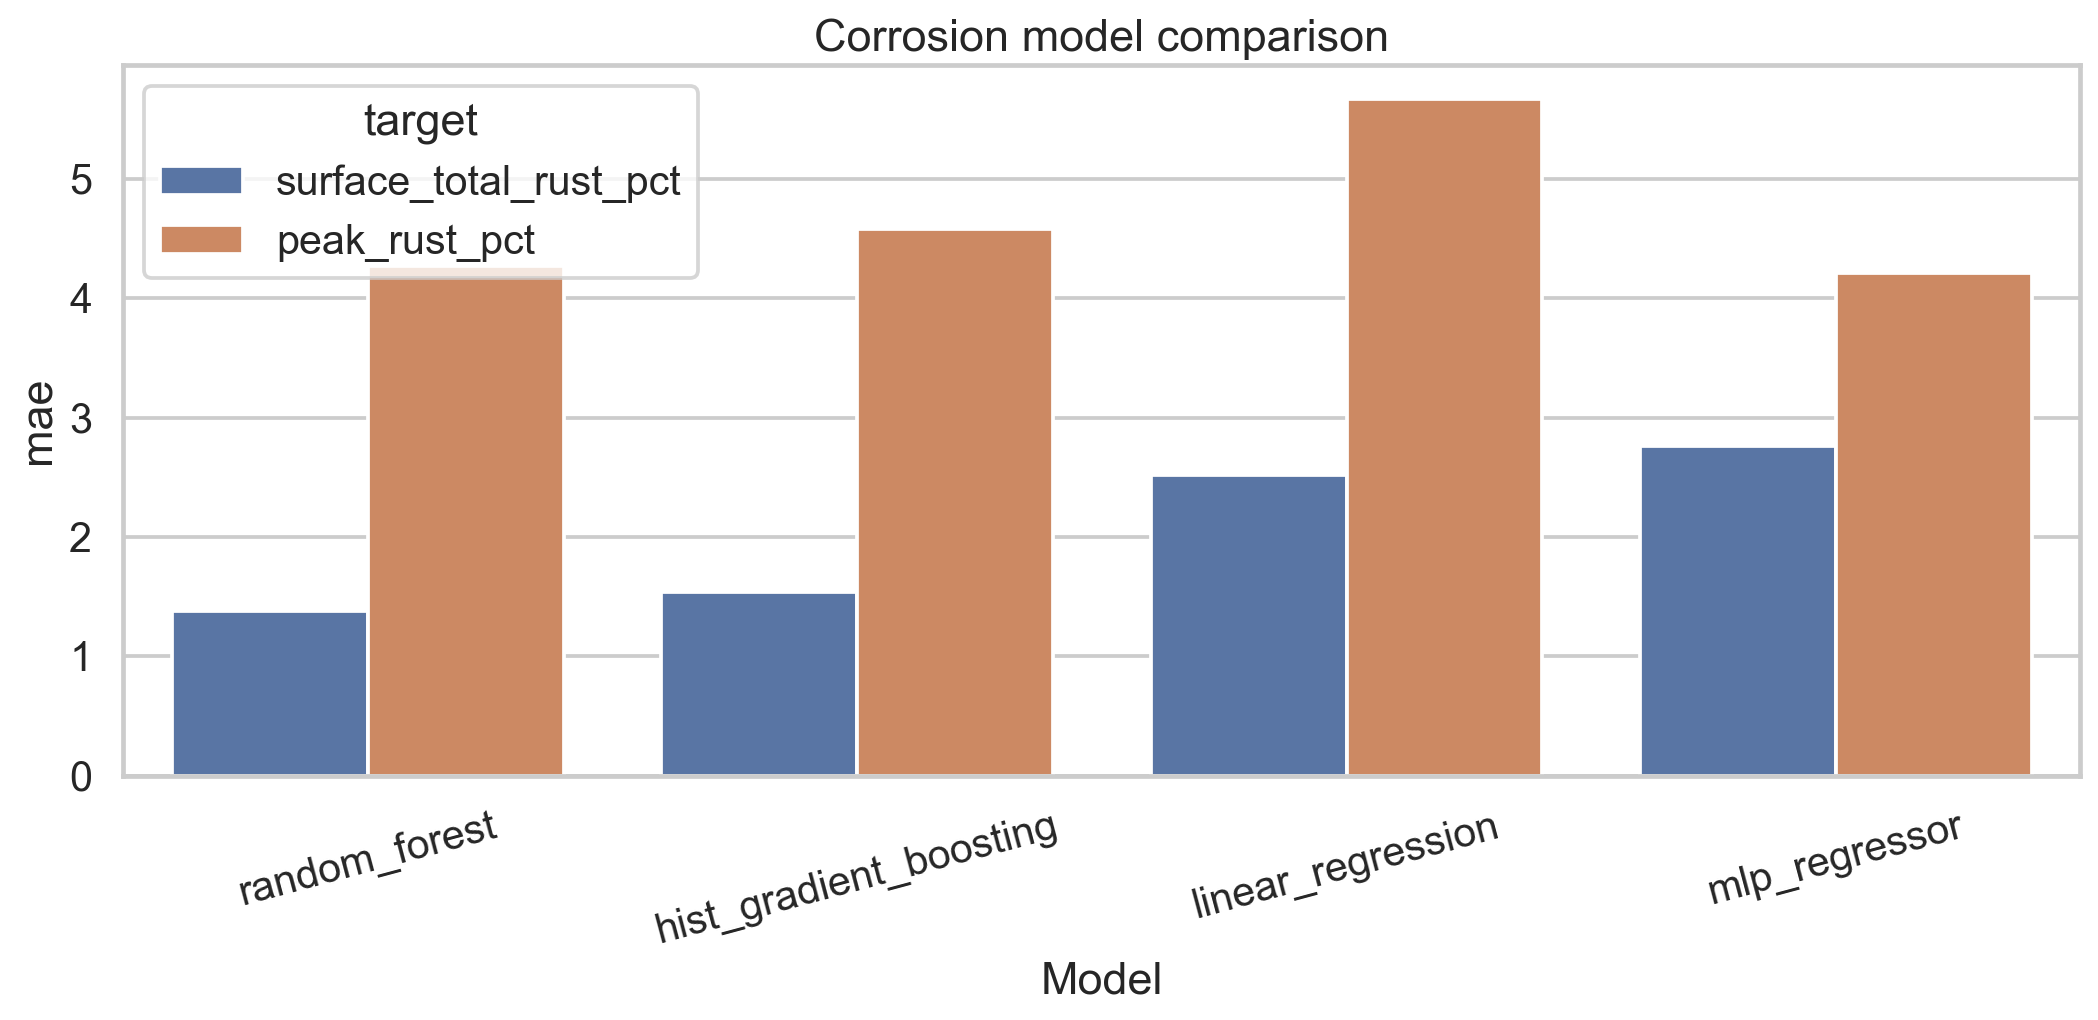
\includegraphics[width=\linewidth]{figures/corrosion_model_mae.png}
    \caption{Grouped specimen-holdout comparison for the visible-corrosion regressors. The figure shows the saved MAE values for the two regression targets under the single grouped split used for model selection. Random Forest is strongest for total rust, while the MLP regressor is strongest for peak rust.}
    \label{fig:corrosion-mae}
\end{figure}

\subsection{Hidden-Damage Modeling}
The hidden-damage stage shows learnable signal, but it is substantially weaker than the visible-corrosion stage. In the grouped specimen-holdout split, the best model for wire-area loss is Random Forest with MAE = 3.90, RMSE = 5.00, and $R^2 = 0.310$. For ultimate load, the best saved MAE is 0.121~kN from Random Forest, although Extra Trees reaches a slightly higher $R^2$ of 0.418 with worse MAE (0.145~kN). These results are best interpreted as feasibility evidence, not as robust structural prediction.

\begin{table}[t]
    \caption{Main Grouped-Holdout Results}
    \label{tab:grouped-results}
    \centering
    \scriptsize
    \setlength{\tabcolsep}{3pt}
    \begin{tabular}{@{}L{0.30\linewidth}L{0.23\linewidth}ccc@{}}
        \toprule
        Task & Best model & MAE & RMSE & $R^2$ \\
        \midrule
        Total visible rust (\%) & Random Forest & 1.38 & 3.14 & 0.646 \\
        Peak visible rust (\%) & MLP Regressor & 4.21 & 6.23 & 0.784 \\
        Wire-area loss (\%) & Random Forest & 3.90 & 5.00 & 0.310 \\
        Ultimate load (kN) & Random Forest & 0.121 & 0.168 & 0.385 \\
        \bottomrule
    \end{tabular}
\end{table}

\subsection{Harder Holdouts and Transfer Checks}
The stricter holdouts make the evidence hierarchy much clearer. For visible corrosion, leave-one-campaign-out still retains positive $R^2$: the best mean results are MAE = 2.10 and $R^2 = 0.582$ for total rust (Random Forest) and MAE = 6.21 with $R^2 = 0.595$ for peak rust (HistGradientBoosting). However, leave-one-treatment-out is much less stable: the best mean $R^2$ becomes negative for both visible corrosion targets, even when MAE remains moderate.

For hidden damage, robustness collapses under both harder views. In leave-one-campaign-out, the best mean wire-loss result is MAE = 12.28 with $R^2 = -0.387$, and the best mean ultimate-load result is MAE = 0.624~kN with $R^2 = -8.356$. In leave-one-treatment-out, the best mean wire-loss result is MAE = 10.76 with $R^2 = -5.481$, and the best mean ultimate-load result is MAE = 0.158~kN with $R^2 = -4.569$. These values show that the structural stage does not transfer robustly across campaign or treatment shifts.

\subsection{Degradation Fits and Screening Outputs}
The degradation stage produced 192 fitted curves and 52{,}416 forecast rows. In the saved outputs, piecewise-linear fits dominate: all 96 structural-target curves are piecewise linear, while the visible-corrosion curves are piecewise linear in 84 of 96 cases and exponential in the remaining 12. Neither linear nor logarithmic fits are selected in the saved \texttt{degradation\_curves.parquet}. Median fit quality is strong for the observed surface targets (median $R^2$ = 0.903 for total rust and 0.916 for peak rust) and weaker for the model-estimated structural targets (median $R^2$ = 0.636 for estimated wire loss and 0.601 for estimated ultimate load).

\begin{table}[t]
    \caption{Selected Degradation Curve Families}
    \label{tab:curve-families}
    \centering
    \small
    \begin{tabular}{lcc}
        \toprule
        Target & Exponential & Piecewise linear \\
        \midrule
        Total visible rust & 8 & 40 \\
        Peak visible rust & 4 & 44 \\
        Estimated wire-area loss & 0 & 48 \\
        Estimated ultimate load & 0 & 48 \\
        \bottomrule
    \end{tabular}
\end{table}

This result is useful descriptively rather than mechanistically. The stage demonstrates that specimen-wise trend fitting is feasible, but it does not establish a physical deterioration law. Figure~\ref{fig:degradation-panel} illustrates both the cross-sectional corrosion progression and representative specimen-wise forecasts used for forward screening.

\begin{figure*}[!t]
    \centering
    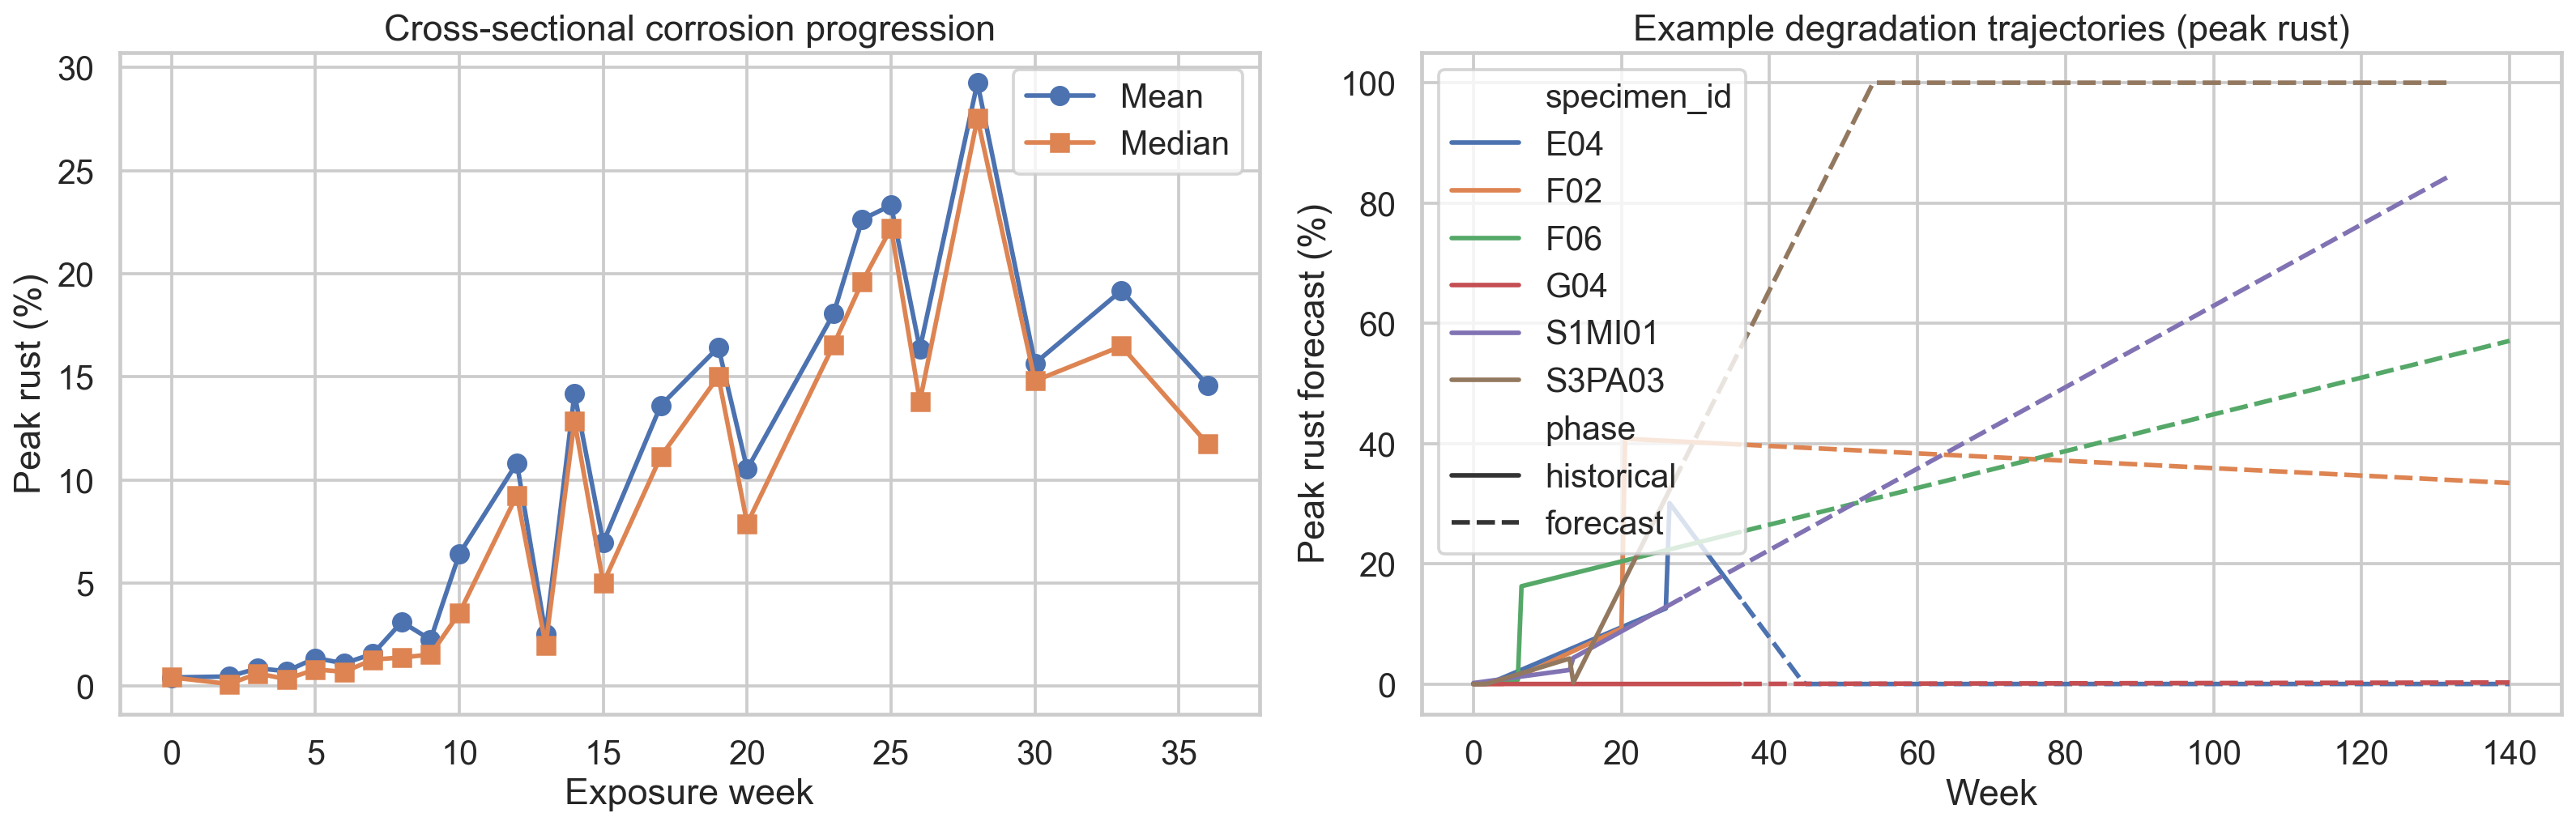
\includegraphics[width=0.94\textwidth]{meeting_report/figures/degradation_examples_panel.png}
    \caption{Representative degradation behavior used by the pipeline. The left panel shows the average and median peak-rust progression across exposure weeks, while the right panel shows example specimen-wise historical and forecast trajectories used for threshold-based screening. Together, the panels illustrate why degradation fitting is treated here as an empirical trend model rather than as a single global deterioration law.}
    \label{fig:degradation-panel}
\end{figure*}

The final remaining-life layer produces screening outputs rather than lifetime predictions. Across the 48 specimens, 33 have finite proxy-RUL estimates, 15 do not cross a threshold within the forecast horizon, 23 already have proxy-RUL equal to 0 weeks, mean proxy-RUL is 5.42 weeks, median proxy-RUL is 0.00 weeks, and maximum proxy-RUL is 55.5 weeks. The corresponding risk distribution is 20 Low, 8 Moderate, 20 High, and 0 Critical.

Among the three criteria used in the default minimum rule, the load threshold is the sole earliest trigger for 16 specimens, the 25\% wire-loss threshold is the sole earliest trigger for 10 specimens, and the remaining 7 finite cases are ties. The health threshold is present in the table but is never the sole earliest trigger in the saved outputs.

\begin{table}[t]
    \caption{Proxy-RUL Summary}
    \label{tab:proxy-rul}
    \centering
    \small
    \begin{tabular}{lr}
        \toprule
        Quantity & Value \\
        \midrule
        Specimens & 48 \\
        Finite proxy-RUL values & 33 \\
        No crossing within horizon & 15 \\
        Zero-week proxy-RUL & 23 \\
        Mean proxy-RUL & 5.42 weeks \\
        Median proxy-RUL & 0.00 weeks \\
        Max proxy-RUL & 55.5 weeks \\
        \bottomrule
    \end{tabular}
\end{table}

Fig.~\ref{fig:risk-distribution} shows the final distribution of screening classes. In this run, the pipeline separated the cohort into low-, moderate-, and high-risk groups, while no specimen reached the critical band.

\begin{figure}[t]
    \centering
    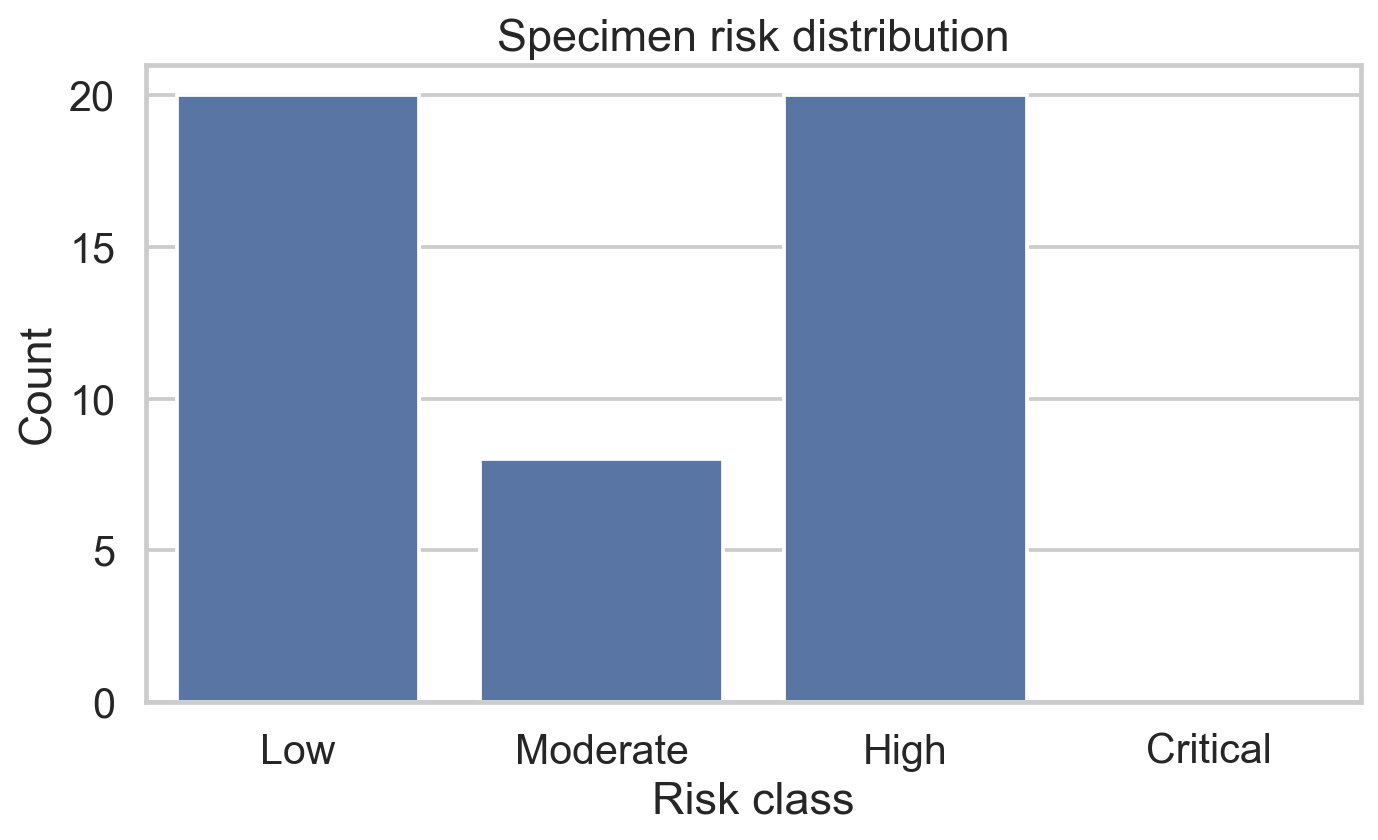
\includegraphics[width=\linewidth]{figures/risk_distribution.png}
    \caption{Distribution of the final risk classes assigned by the proxy-RUL screening stage. In this run, the cohort separates into low-, moderate-, and high-risk groups, while no specimen enters the critical band under the chosen screening thresholds.}
    \label{fig:risk-distribution}
\end{figure}

\section{Discussion}
The strongest validated result of the repository is visible-corrosion modeling. That stage is dense-label, image-driven, and leakage-aware at the specimen level. The grouped split shows substantial predictive power, and the campaign holdout still retains useful signal.

The hidden-damage stage is more limited for two separate reasons. First, it is supervised on only 48 late-stage rows. Second, it is not an end-to-end continuation of the image-only corrosion stage: the saved damage models use manual corrosion labels and metadata in addition to selected image descriptors. The structural layer should therefore be described as a mixed-input feasibility model rather than as direct internal-state recovery from images.

The degradation stage is useful, but it should not be overinterpreted. It selects the curve family with minimum in-sample RMSE, imposes no monotonicity or physics constraint, and fits structural trajectories to model-generated hidden states. Good historical fit is therefore not equivalent to validated future structural forecasting.

The proxy-RUL stage is best understood as a downstream screening layer. It is useful precisely because the repository does not pretend to do more than the data support. The outputs answer a threshold-status question under a finite forecast horizon; they do not estimate experimentally observed failure time.

The main achievement of the study is therefore not a single score, but a coherent corrosion-to-condition workflow with clear evidence boundaries: direct surface evidence first, mixed-input latent structural estimation second, empirical degradation fitting third, and screening-only outputs last.

\section{Threats to Validity}
Several limitations directly affect interpretation:
\begin{enumerate}
    \item sparse structural supervision, because the structural targets are observed only once per specimen;
    \item campaign dependence, because campaign, mesh count, NaCl level, ageing duration, and week horizon move together and can act as surrogate variables;
    \item treatment imbalance, because structural rows are highly uneven across treatments;
    \item no true failure times, which makes supervised remaining-life prediction impossible;
    \item downstream manual-label dependence, because the damage stage uses manual corrosion labels rather than only upstream predicted corrosion states;
    \item model-on-model trajectories, because hidden-damage and load curves are fitted to full-table estimated states rather than repeated structural measurements;
    \item no monotonicity or mechanistic constraint in curve fitting, which can produce non-physical tails;
    \item category-definition ambiguity, because the repository stores ordinal corrosion categories but not the quantitative cutoffs behind the 1--5 scale.
\end{enumerate}

\section{Conclusion}
This paper documents the repository as an interpretable feasibility pipeline rather than a final prognostic system. The implemented workflow reconstructs specimen histories, extracts 91 corrosion-focused image features, performs image-only visible-corrosion modeling, estimates hidden structural quantities with mixed inputs, fits specimen-level degradation curves, and converts forecasted threshold crossing into proxy-RUL and risk classes.

The strongest validated evidence lies in the visible-corrosion stage. The hidden-damage stage remains feasible but structurally weak, and the proxy-RUL layer is screening-only by design. The most defensible summary is therefore simple: repeated corrosion images support a useful corrosion-to-condition workflow, but sparse structural supervision sharply limits what can be claimed about hidden damage and remaining life.

\end{document}
